%
\documentclass[12pt]{article}

% usual packages
\usepackage{fullpage}
\usepackage{setspace}
\usepackage{graphicx}
\usepackage{float}
\usepackage{amsmath}
\usepackage{amsfonts}
\usepackage{amssymb}

% bibliography and references
\usepackage{natbib}
\bibpunct{(}{)}{;}{a}{}{,}

% set paragraph spacing the way I like
\parskip=0pt
\parindent=20pt

% remove indent from footnotes
%\usepackage[hang,flushmargin]{footmisc}

% style font beneath figures
\usepackage[labelfont={bf}, margin=0cm, font=small, skip=0pt]{caption}

% create footnote command so that my name
% has an asterisk rather than a one.
\long\def\symbolfootnote[#1]#2{\begingroup%
\def\thefootnote{\fnsymbol{footnote}}\footnote[#1]{#2}\endgroup}

% body font
\usepackage[T1]{fontenc}
\usepackage{newtxtext,newtxmath}


% pdf meta data and link styling
\usepackage{hyperref}
\hypersetup{
 pdftitle={Estimating Logit Models with Small Samples}, % title
 pdfauthor={Kelly McCaskey and Carlisle Rainey}, % author
 pdfkeywords={logit}{probit}{logistic regression} {small sample} {bias},
 pdfnewwindow=true, % links in new window
 colorlinks=true, % false: boxed links; true: colored links
 linkcolor=black, % color of internal links
 citecolor=black, % color of links to bibliography
 filecolor=black, % color of file links
 urlcolor=blue % color of external links
}

%% enable comments in pdf
%\newcommand{\kelly}[1]{\textcolor{blue}{#1}}
%\newcommand{\carlisle}[1]{\textcolor{magenta}{#1}}


\begin{document}

\begin{appendix}
\begin{center}
{\LARGE Appendix}\\
\vspace{3mm}
{\large Estimating Logit Models with Small Samples}\\\vspace{2mm}

\vspace{10mm}

Carlisle Rainey\symbolfootnote[2]{Carlisle Rainey is Associate Professor of Political Science, Florida State University, 540 Bellamy, Tallahassee, FL, 32306. (\href{mailto:crainey@fsu.edu}{crainey@fsu.edu}).}

\vspace{3mm}

Kelly McCaskey\symbolfootnote[2]{Kelly McCaskey is Operations Analyst at Accruent, 11500 Alterra Parkway, \#110, Austin, TX, 78758 (\href{mailto:kmccaskey@accruent.com}{kmccaskey@accruent.com}).}

\end{center}

\vspace{10mm}


\section{PML Estimation in R}\label{sec:pmle-in-R}

This example code is available at \href{https://github.com/kellymccaskey/small/blob/master/stata/example.do}{https://github.com/kellymccaskey/small/blob/master/stata/example.do} and \href{https://github.com/kellymccaskey/small/blob/master/R/example.R}{https://github.com/kellymccaskey/small/blob/master/R/example.R}.

\begin{footnotesize}
\begin{verbatim}

# load data from web
library(readr)  # for read_csv()
weisiger <- read_csv([redacted])

# quick look at data
library(dplyr)  # for glimpse()
glimpse(weisiger)

# model formula
f <- resist ~ polity_conq + lndist + terrain +
  soldperterr + gdppc2 + coord

# ----------------------------- #
# pmle with the logistf package #
# ----------------------------- #

# estimate logit model with pmle
library(logistf)  # for logistf()
m1 <- logistf(f, data = weisiger)

# see coefficient estimates, confidence intervals, p-values, etc.
summary(m1)

# logistf does **NOT** work with texreg package
library(texreg)
screenreg(m1)

# see help file for more
help(logistf)

# --------------------------- #
# pmle with the brglm package #
# --------------------------- #

# estimate logit model with pmle
library(brglm)  # for brglm()
m2 <- brglm(f, family = binomial, data = weisiger)

# see coefficient estimates, standard errors, p-values, etc.
summary(m2)

# brglm works with texreg package
screenreg(m2)

# see help file for more
help(brglm)
\end{verbatim}
\end{footnotesize}

\section{PML Estimation in Stata}\label{sec:pmle-in-stata}

This example code is available at [redacted].%\href{https://github.com/kellymccaskey/small/blob/master/stata/example.do}{https://github.com/kellymccaskey/small/blob/master/stata/example.do}.

\noindent The example data used is available at [redacted].%\href{https://github.com/kellymccaskey/small/blob/master/stata/GE.dta}{https://github.com/kellymccaskey/small/blob/master/stata/ge.csv}.


\begin{footnotesize}
\begin{verbatim}
* set working directory and load data
* data can be found at [redacted] 
cd "your working directory"
insheet using "ge.csv", clear

* install firthlogit
ssc install firthlogit

* estimate logit model with pmle
* see coefficient values, standard errors, p-values, etc.
firthlogit court dq cr pc ag sp pe cc ap dc st sg

* see help file for more
help firthlogit

\end{verbatim}
\end{footnotesize}


\section{Additional Simulation Results}\label{sec:app-sims}

\subsection{Expected Value}

\begin{figure}[H]
\begin{center}
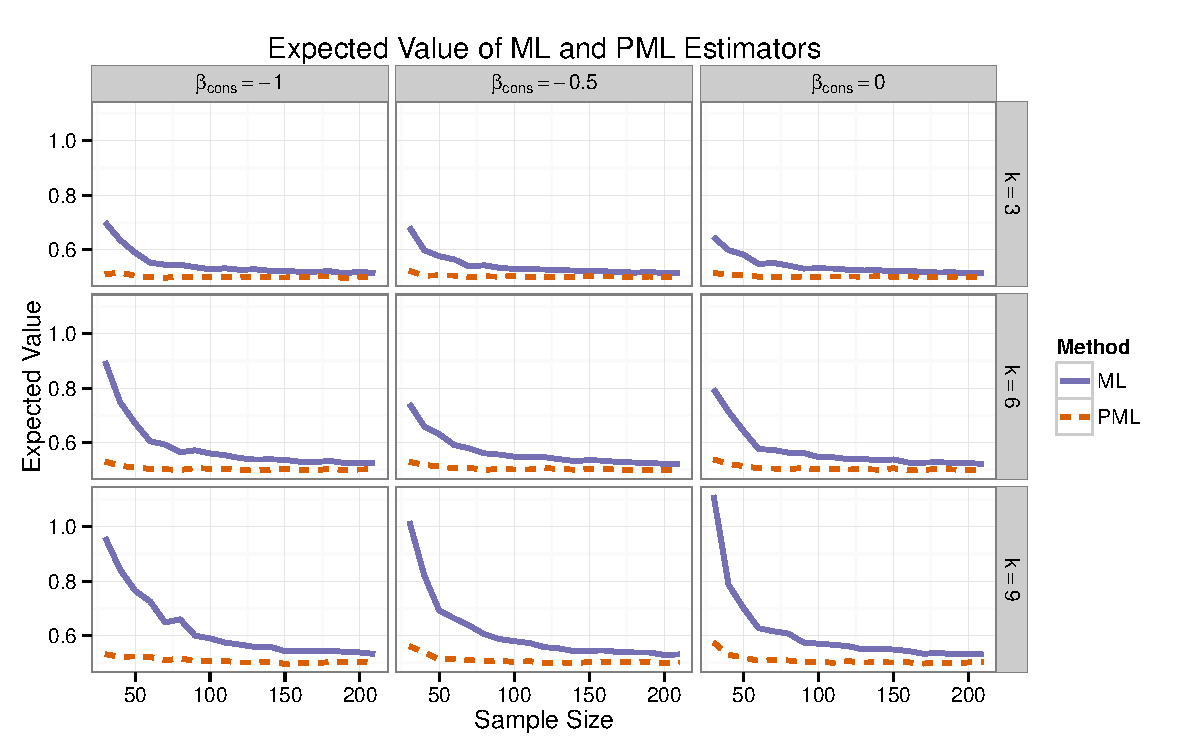
\includegraphics[width = \textwidth]{figs/sims-ev.pdf}
\caption{This figure shows the expected value of $\hat{\beta}^{mle}$ and $\hat{\beta}^{pmle}$. The true value is $\beta = 0.5$.}\label{fig:ev}
\end{center}
\end{figure}

\subsection{Bias}

\begin{figure}[H]
\begin{center}
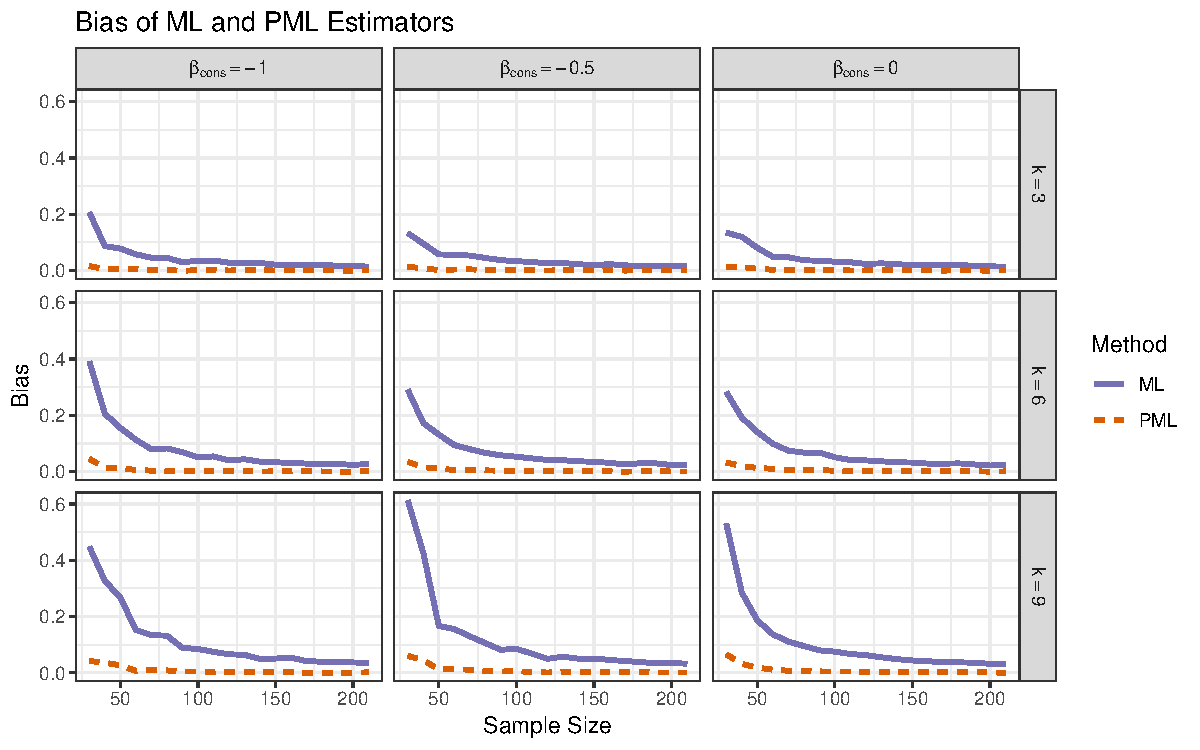
\includegraphics[width = \textwidth]{figs/sims-bias.pdf}
\caption{This figure shows the bias of $\hat{\beta}^{mle}$ and $\hat{\beta}^{pmle}$.}\label{fig:bias}
\end{center}
\end{figure}

\subsection{Variance Inflation}

\begin{figure}[H]
\begin{center}
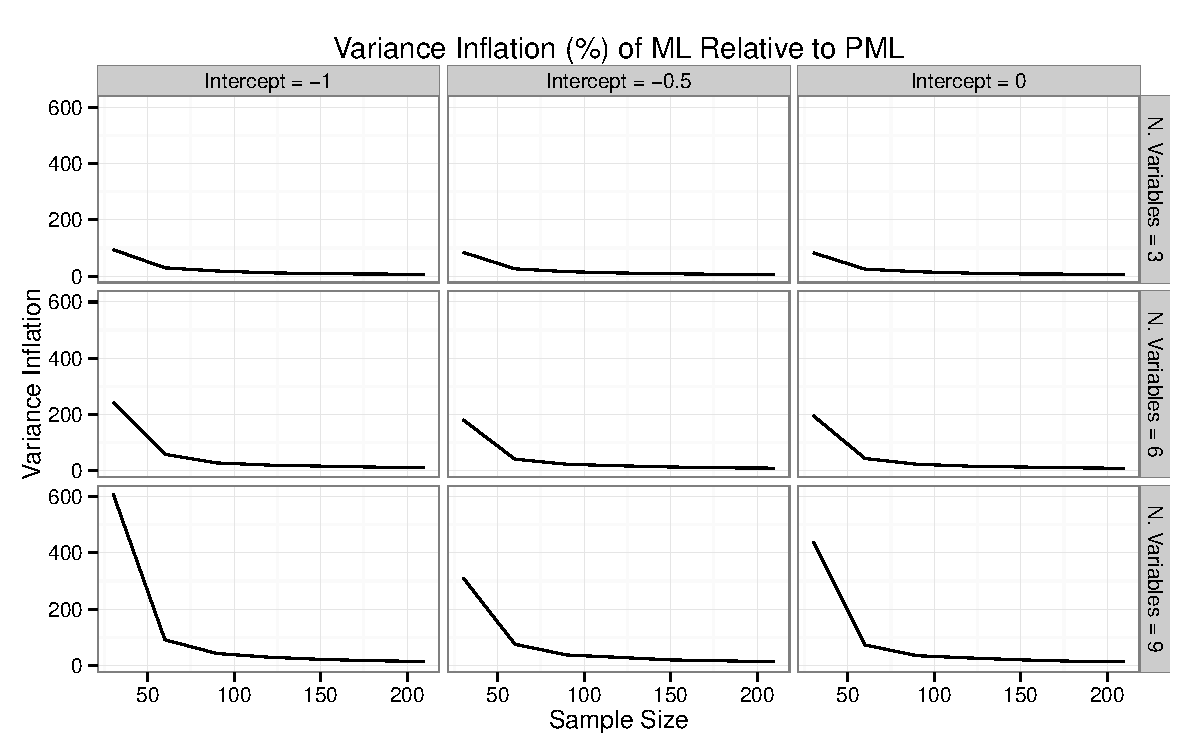
\includegraphics[width = \textwidth]{figs/sims-var-infl.pdf}
\caption{This figure shows the percent inflation in the variance of $\hat{\beta}^{mle}$ compared to $\hat{\beta}^{pmle}$.}\label{fig:var-infl}
\end{center}
\end{figure}

\section{Re-Analysis of \cite{Weisiger2014}}\label{app:weisiger}

Weisiger describes how, after the official end of the war, violence sometimes continues in the form of guerrilla warfare.
He argues that resistance is more likely when conditions are favorable for insurgency, such as difficult terrain, a occupying force, or a pre-war leader remains at-large in the country.

Weisiger's sample consists of 35 observations (with 14 insurgencies).
We reanalyze Weisiger's data using a logit model to show the substantial difference between the biased, high-variance ML estimates and the nearly unbiased, low-variance PML estimates.\footnote{Specifically, we reanalyze the Model 3 in Weisiger's Table 2 (p. 14).
In the original analysis, Weisiger uses a linear probability model.
He writes that ``I [Weisiger] make use of a linear probability model, which avoids problems with separation but introduces the possibility of non-meaningful predicted probabilities outside the [0,1] range'' (p. 11).
As he notes, predictions outside the $[0, 1]$ interval pose a problem for interpreting the linear probability model.
In these data for example, the linear probability model estimates a probability of 1.41 of insurgency in one case.
In another, it estimates a probability of -0.22.
Overall, 25\% of the estimated probabilities based on the linear probability model are larger than one or less than zero.
Of course, these results are nonsense.
However, because of the well-known small-sample bias, methodologists discourage researchers from using a logit model with small samples.
The PML approach, though, solves the problem of bias as well as nonsense predictions.} Prior to estimation, we standardize the continuous variables to have mean zero and standard deviation one-half and binary variables to have mean zero \citep{Gelman2008}.
Figure \ref{fig:weisiger-coefs} shows the coefficient estimates and 90\% confidence intervals using ML and PML.
Notice that the PML estimates are substantially smaller in many cases.
Although the coefficient for terrain only changes by 16\%, each of the remaining coefficients changes by more than 45\%!
The coefficient for per capita GDP shrinks by more the 60\% and the coefficient for occupying force density grows by nearly 100\%.
Also notice that the PML standard errors are much smaller--the ML estimates for the coefficients of a coordinating leader and for the intercapital distance fall outside the PML 90\% confidence interval.
On average, the PML confidence intervals are about half as wide as the ML confidence intervals.

\begin{figure}[h]
\begin{center}
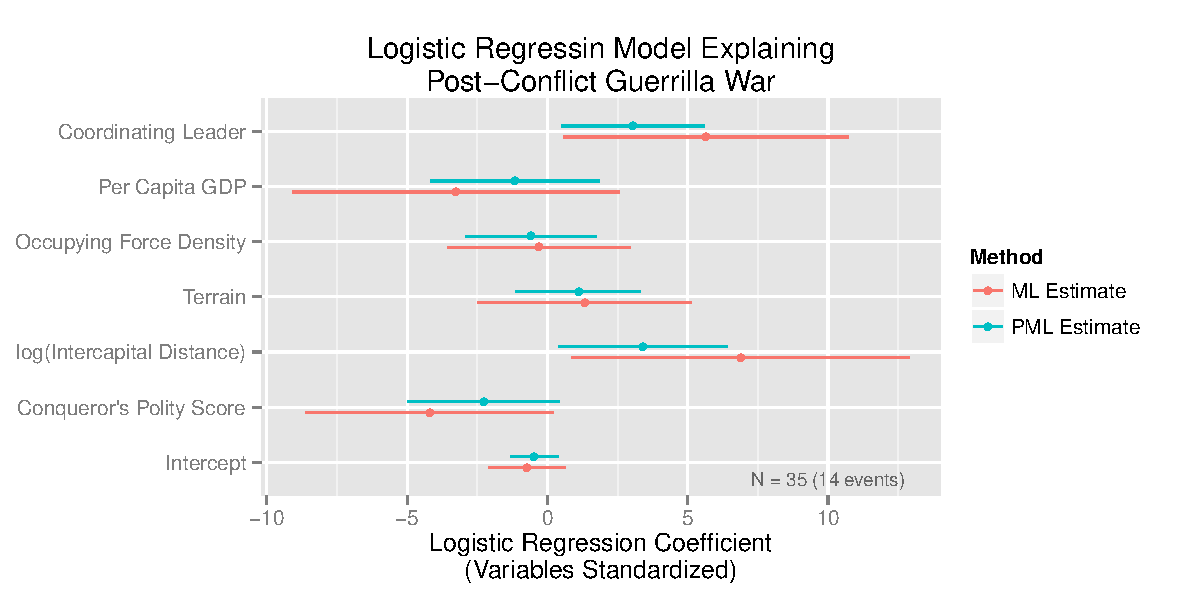
\includegraphics[width = \textwidth]{figs/weisiger-coefs.pdf}
\caption{This figure shows the coefficients for a logit model model estimated explaining post-conflict guerrilla war estimated with ML and PML.
Notice that the PML estimates and confidence intervals tend to be much smaller than the ML estimates and confidence intervals.}\label{fig:weisiger-coefs}
\end{center}
\end{figure}

Because we do not know the true model, we cannot know which of these sets of coefficients is better.
However, we can use out-of-sample prediction to help adjudicate between these two methods.
We use leave-one-out cross-validation and summarize the prediction errors using Brier and log scores, for which smaller values indicate better predictive ability.\footnote{The Brier score is calculated as $\sum_{i = 1}^n (y_i - p_i)^2$, where $i$ indexes the observations, $y_i \in \{0, 1\}$ represents the actual outcome, and $p_i \in (0, 1)$ represents the estimated probability that $y_i = 1$.
The log score as $-\sum_{i = 1}^n log(r_i)$, where $r_i = y_i p_i + (1 - y_i)(1 - p_i)$.
Notice that because we are logging $r_i \in [0, 1]$, $\sum_{i = 1}^n log(r_i)$ is always negative and smaller (i.e., more negative) values indicate worse fit.
We choose to take the negative of $\sum_{i = 1}^n log(r_i)$, so that, like the Brier score, larger values indicate a worse fit.}
The ML estimates produce a Brier score of 0.14, and the PML estimates lower the Brier score by 14\% to 0.12.
The ML estimates produce a log score of 0.58, while the PML estimates lower the log score by 34\% to 0.38.
The PML estimates outperform the ML estimates for both approaches to scoring, and
this provides good evidence that the PML estimates better capture the data generating process.

Because we are using a logit model, we might be more interested in \textit{functions} of the coefficients than in the coefficients themselves.
For an example, we focus on Weisiger's hypothesis that there will be a greater chance of resistance when the pre-conflict political leader remains at large in the conquered country.
Setting all other explanatory variables at their sample medians, we calculated the predicted probabilities, the first difference, and the risk ratio for the probability of a post-conflict guerrilla war as countries gain a coordinating leader.
Figure \ref{fig:weisiger-qis} shows the estimates of the quantities of interest.

\begin{figure}[h]
\begin{center}
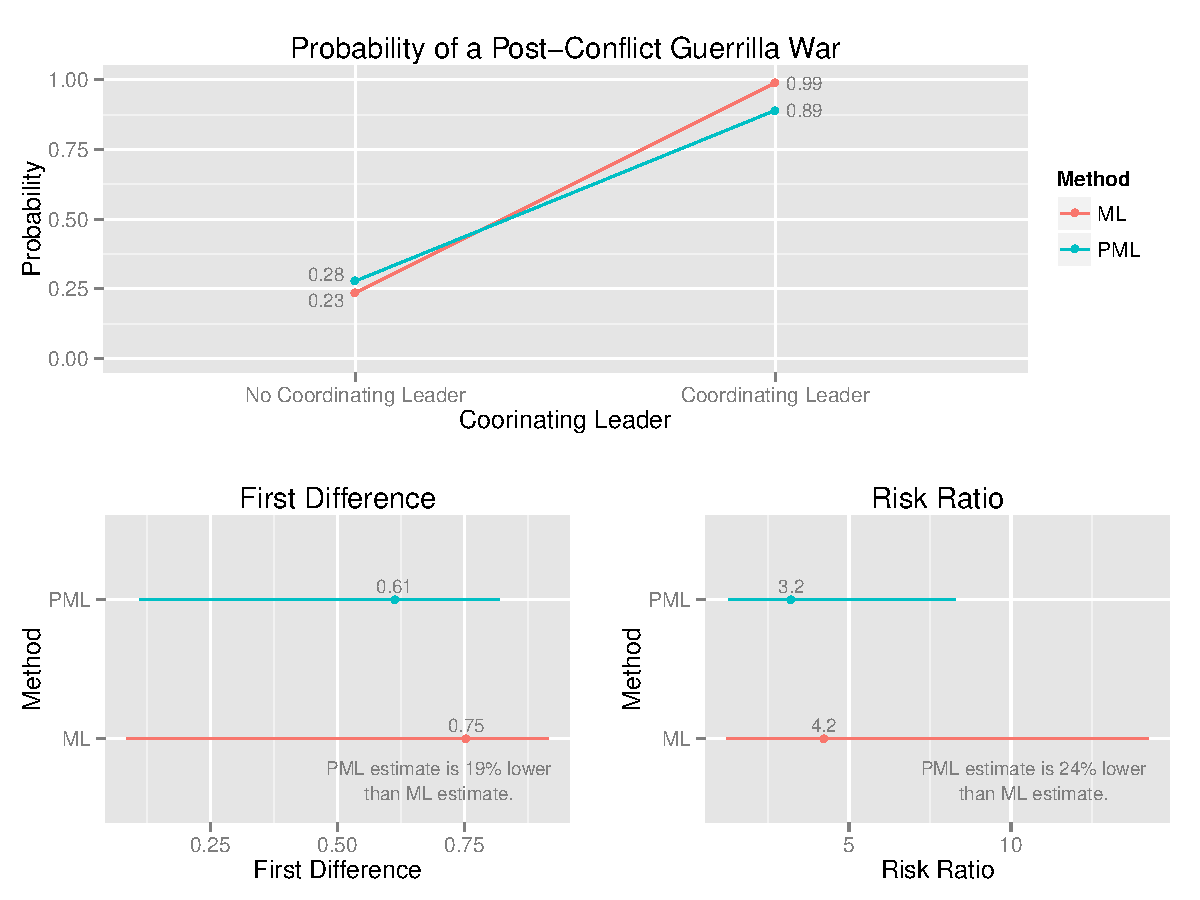
\includegraphics[width = \textwidth]{figs/weisiger-qis.pdf}
\caption{This figure shows the quantities of interest for the effect of a coordinating leader on the probability of a post-conflict guerrilla war.}\label{fig:weisiger-qis}
\end{center}
\end{figure}

PML pools the estimated probabilities toward one-half, so that when a country lacks a coordinating leader, ML suggests a 23\% chance of rebellion while PML suggests a 28\% chance.
On the other hand, when country \textit{does have} a coordinating leader, ML suggests a 99\% chance of rebellion, but PML lowers this to 89\%.
Accordingly, PML suggests smaller effect sizes, whether using a first difference or risk ratio.
PML shrinks the estimated first difference by 19\% from 0.75 to 0.61 and the risk ratio by 24\% from 4.2 to 3.2.

\singlespace
\normalsize
\bibliographystyle{apsr_fs}
\bibliography{bibliography.bib}

\end{appendix}


\end{document}
